\section*{Anexo E. Cuenta individual \textit{equity-linked}}
\label{sec:anexo-equity}

En la trayectoria 1, el cargo del $2\%$ deja $98\,000$ para invertir y el del $3\%$ deja $97\,000$, de modo que con un rendimiento del $12{,}5344\%$ el primer año cierra en $110\,283{,}67$ y $109\,158{,}32$, respectivamente. Al cierre del quinto año, los tres saldos quedan por debajo de su garantía y el NPV es negativo en los dos casos con garantía de $110\,000$.

\begin{table}[htbp]
\centering
\small
\setlength{\tabcolsep}{4pt}
\begin{tabular}{@{}rrrrrrr@{}}
\toprule
Año & Tasa de cargo & Rendimiento & Saldo inicial & Cargo & Saldo final & VP de cargo \\
\midrule
1 & 2\% & 12,53\% & 100\,000,00 & 2\,000,00 & 110\,283,67 & 2\,000,00 \\
2 & 2\% & -11,48\% & 110\,283,67 & 2\,205,67 & 95\,669,50 & 2\,050,47 \\
3 & 2\% & 6,28\% & 95\,669,50 & 1\,913,39 & 99\,641,88 & 1\,653,39 \\
4 & 2\% & 2,77\% & 99\,641,88 & 1\,992,84 & 100\,350,34 & 1\,600,42 \\
5 & 2\% & -5,82\% & 100\,350,34 & 2\,007,01 & 92\,616,64 & 1\,497,70 \\
1 & 3\% & 12,53\% & 100\,000,00 & 3\,000,00 & 109\,158,32 & 3\,000,00 \\
2 & 3\% & -11,48\% & 109\,158,32 & 3\,274,75 & 93\,727,02 & 3\,044,32 \\
3 & 3\% & 6,28\% & 93\,727,02 & 2\,811,81 & 96\,622,63 & 2\,429,72 \\
4 & 3\% & 2,77\% & 96\,622,63 & 2\,898,68 & 96\,316,68 & 2\,327,89 \\
5 & 3\% & -5,82\% & 96\,316,68 & 2\,889,50 & 87\,986,76 & 2\,156,24 \\
\bottomrule
\end{tabular}

\caption{Saldos y cargos anuales de la trayectoria 1, en unidades monetarias, con una proyección común para ambas garantías con cargo del $2\%$.}
\label{tab:equity-trayectoria-anual}
\end{table}

\begin{table}[htbp]
\centering
\small
\begin{tabular}{@{}lrrr@{}}
\toprule
Garantía / cargo & 100\,000 / 2\% & 110\,000 / 2\% & 110\,000 / 3\% \\
\midrule
Saldo al cierre del año 5 & 92\,616,64 & 92\,616,64 & 87\,986,76 \\
Complemento al vencimiento & 7\,383,36 & 17\,383,36 & 22\,013,24 \\
VP de cargos & 8\,801,98 & 8\,801,98 & 12\,958,18 \\
VP del complemento & 5\,118,63 & 12\,051,29 & 15\,261,02 \\
NPV del proveedor & 3\,683,35 & -3\,249,31 & -2\,302,84 \\
\bottomrule
\end{tabular}

\caption{Cierre de la cuenta y NPV del proveedor en la trayectoria 1, en unidades monetarias.}
\label{tab:equity-trayectoria}
\end{table}

\begin{figure}[!htbp]
\centering
\graphicspath{{resultados/equity_linked/}}
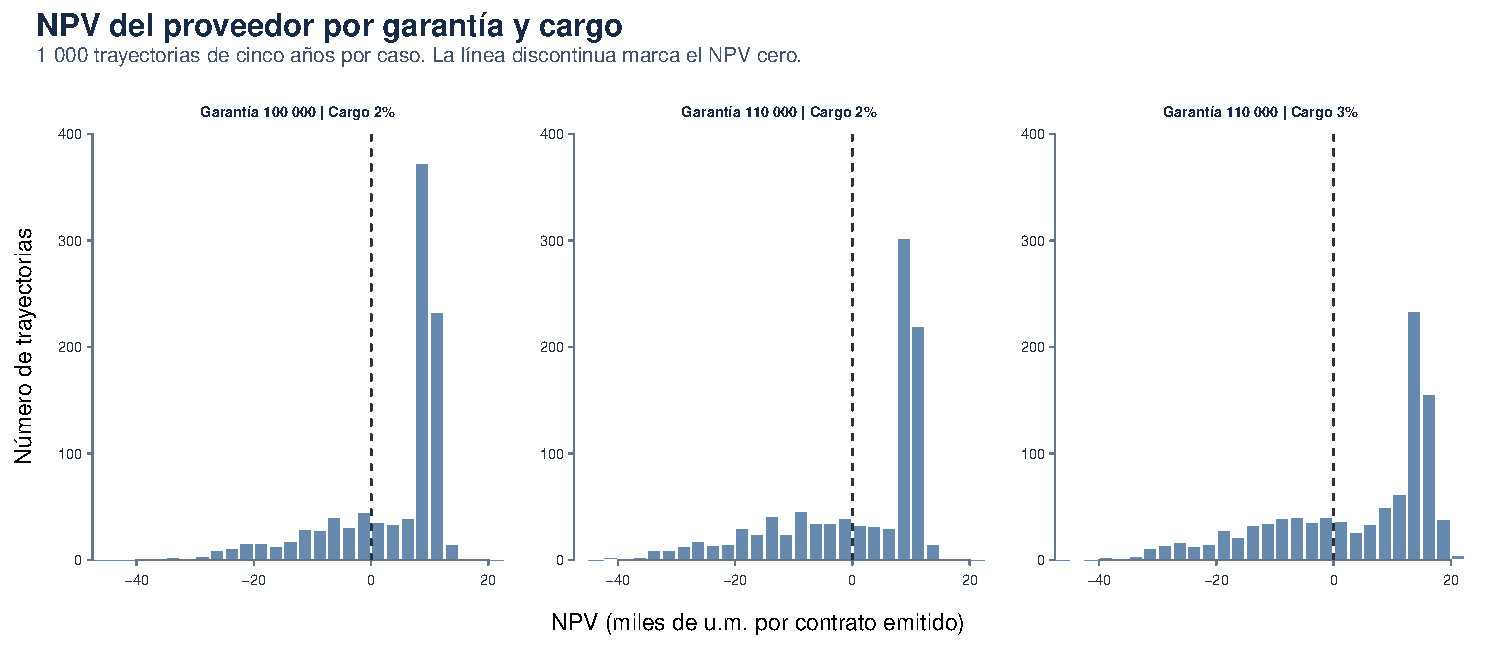
\includegraphics[width=0.95\textwidth]{histograma_npv.pdf}
\caption{Distribución del NPV por caso, con las mismas escalas e intervalos de $2\,500$ unidades monetarias.}
\label{fig:equity-npv}
\end{figure}
